\section {Bias Variance trade off}
The Bias variance trade off is an important part of modelling and if not done right accuracy of the model will not perform well. We would like a model that that capture the structure of the data but also works well on unseen data and we can't get both. A model with high variance represent the training data well, but are at risk of overfitting hence also capturing the noise in training data. On the other hand models with high bias produce simpler models underfit their training data therefore failing to capture structure of the data.

\begin{figure}[h]
	\centering
	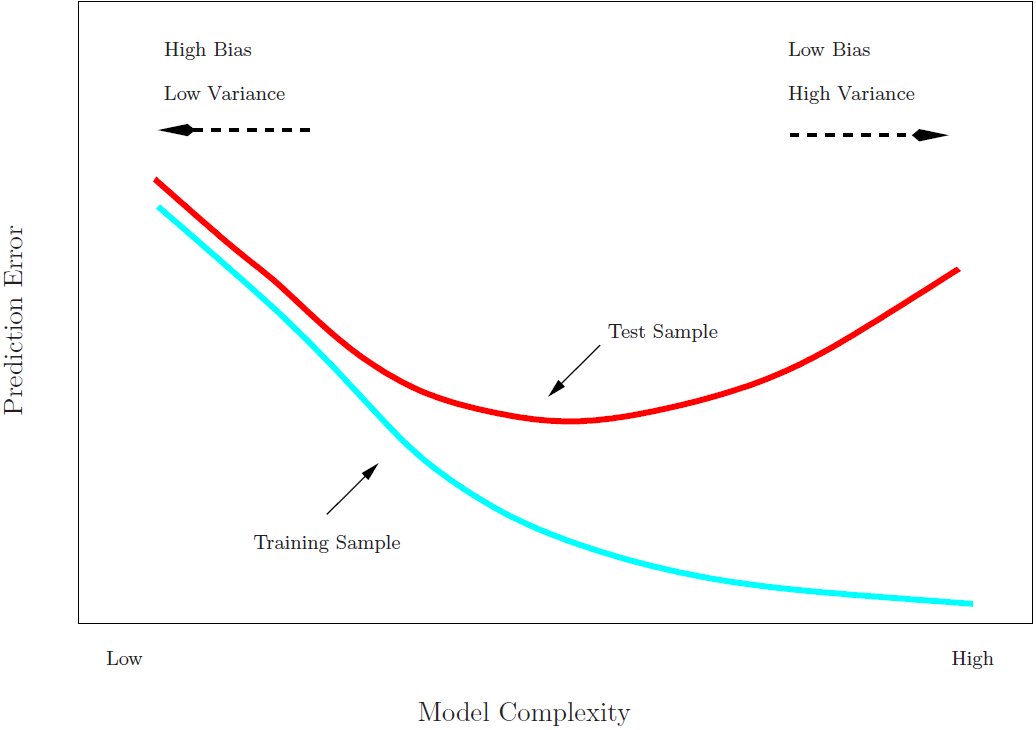
\includegraphics[width=0.5\linewidth]{crossValidation/biasVariance}
	\caption{Bias Variance trade off}
	\label{fig:biasvariance}
\end{figure}
